\chapter{Die Skelettierung}
\Autor{Sandra Schröder}\\
Ein Skelett ist ein nützlicher Deskriptor, um Informationen über die Region und den Rand eines Objektes kompakt und effizient
zu kodieren. Es gibt die wesentlichen Grundzüge eines Objektes wieder.\\
Dieses Kapitel beschreibt bekannte Konzepte und Verfahren zur Skelettierung im Bereich der Bildverarbeitung.\\
Zwei Verfahren sind im Rahmen der Projektarbeit besonders wichtig: Das \emph{Thinning} (deutsch: Verdünnung) und die \emph{Distanztransformation}. \\
Um die Übersicht über die weiteren grundlegenden Verfahren und Konzepte zu vervollständigen, werden diese in einem separaten 
Abschnitt kurz vorgestellt.
\section{Thinning}
\Autor{Johannes Böhler}\\
Das Thinning bezeichnet eine Kategorie von Methoden zur Skelettierung von 2D sowie 3D Objekten. In dieser Projektarbeit ist der Fokus ausschliesslich auf die 2D Skelettierung gerichtet, da die Kinect kein vollkommenes 3D Modell eines Objektes liefert. Sie erfasst das Objekt lediglich aus einem Blickwinkel, desshalb erhält man nur ein 2,5 dimensionales Modell. Es werden nur Tiefeninformationen bezüglich der Seite des Objektes, welche der Kinect zugewendet ist bereitgestellt. Die  Tiefeninformationen der Rückseite bleiben verborgen. Um ein vollständiges 3D Modell zu erhalten müssten mindestens 2 Kinects verwendet werden und die Informationen beider Geräte zusammengeführt und vereinheitlicht werden. 

Alle Thinning Algorithmen verbindet das iterative Abtragen des Musters oder der Oberfläche.

\section{Distanztransformation}
\Autor{Sandra Schröder}\\\\
%Sandra: Theorie über Skelettierung mit der Distanztransformation
...\\
Die Distanztransformation eines Binärbildes enthält Informationen über den Abstand der Objektpixel zum Rand des Objekts. Die
Pixel die im Objekt beziehungsweise in Objektregionen mittig liegen, besitzen den größten Abstand zum Rand relativ zu den 
umgebenden Pixeln. Die Pixel mit dem größten Abstand sind dementsprechend die hellsten Pixel in der Distancemap. 
Die Distancemap beschreibt ein Grauwertgebirge, wobei sich der Gebirgskamm in der Mitte des Objektes befindet.
\label{sec:distanztransformation}
\begin{figure}[h]
	\centering
	\begin{minipage}{5cm}
		\centering
		
\includegraphics[width=1.0\linewidth]{./fig/person.jpg}
		\label{fig:beispiel_person}
	\end{minipage}
	\hspace{3cm}
	\begin{minipage}{5cm}
		\centering
		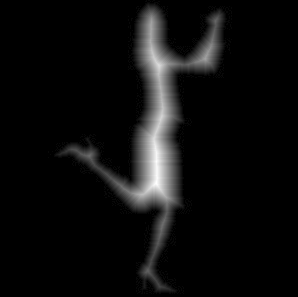
\includegraphics[width=1.0\linewidth]{./fig/distance_map_beispiel}
		\label{fig:distance_map_beispiel}
	\end{minipage}
	\caption{Distance Map TODO: nähere Beschreibung}
\end{figure}
\section{Weitere Verfahren}
\Autor{Christopher Kroll}